\documentclass[a4paper,english,12pt]{article}   	% use }amsart} instead of }article} for AMSLaTeX format
\usepackage{%
	amsfonts,%
	amsmath,%	
	amssymb,%
	amsthm,%
	bbm,%
	biblatex,%
	caption,%
	color,%
	enumerate,%
	epsfig,%
	epstopdf,%
	geometry,%
	graphicx,%
	hyperref,%
	latexsym,%
	mathtools,%
	multicol,%
	pgf,%
	%pgfplots%
	%pgfplotstable,%
	pgfpages,%
	proof,%
	psfrag,%
	subfigure,%	
	tikz,%
	ulem,%
	url%
}

\usepackage[mathscr]{eucal}
\usepgflibrary{shapes}
\usetikzlibrary{%
  arrows,%
	backgrounds,%
	chains,%
	decorations.pathmorphing,% /pgf/decoration/random steps | erste Graphik
	decorations.text,%
	matrix,%
  positioning,% wg. " of "
  fit,%
	patterns,%
  petri,%
	plotmarks,%
  scopes,%
	shadows,%
  shapes.misc,% wg. rounded rectangle
  shapes.arrows,%
	shapes.callouts,%
  shapes%
}

\theoremstyle{plain}
\newtheorem{thm}{Theorem}[section]
\newtheorem{lem}[thm]{Lemma}
\newtheorem{prop}[thm]{Proposition}
\newtheorem{cor}[thm]{Corollary}

\theoremstyle{definition}
\newtheorem{defn}[thm]{Definition}
\newtheorem{conj}[thm]{Conjecture}
\newtheorem{exmp}[thm]{Example}
\newtheorem{assum}[thm]{Assumptions}

\theoremstyle{remark}
\newtheorem{rem}{Remark}
\newtheorem{note}{Note}

\newcommand{\norm}[1]{\left\lVert#1\right\rVert}
\newcommand{\tr}{\operatorname{tr}}
\newcommand{\Real}{\mathbb{R}}

\makeatletter
\def\th@plain{%
  \thm@notefont{}% same as heading font
  \itshape % body font
}
\def\th@definition{%
  \thm@notefont{}% same as heading font
  \normalfont % body font
}
\makeatother
\date{}
\geometry{letterpaper}                   		% ... or a4paper or a5paper or ...


\title{Lecture 12 : Topological Spaces}
\author{}

\begin{document}
\maketitle
%\section{}
%\subsection{}
\section{Topological Spaces}
\begin{defn}[Topology] A \textbf{topology} on a set $X$ is a collection $\T$ of subsets of $X$ having the following properties
\begin{enumerate}
\item $\emptyset$ and $X$ are in $\T$.
\item The union of the elements of any sub-collection of $\T$ is in $\T$.
\item The intersection of any finite sub-collection of $\T$ is in $\T$. A set $X$ for which a topology $\T$ has been specified is called a \textbf{topological space $(X,\T)$}.
\end{enumerate}
\end{defn}
\begin{defn}[Open Set] If $X$ is a topological space with topology $\T$, we say that a subsets $U$ of $X$ is an \textbf{open set} of $X$ if $U$ belongs to the collection of $\T$.
\end{defn}
\begin{exmp} 
 Let $X$ be any set, then its power set $\mathcal{P}(X)$ is a topology and is called as \textbf{discrete topology}.  While topology $\T =\{\emptyset,X\}$ is called \textbf{indiscrete topology} or \textbf{trivial topology}.
\end{exmp}
\begin{exmp} 
 Let $X$ be a set, and let $\T_f = \{U\subseteq X : X \setminus U\text{ is finite or }X \setminus U= X\}$. Prove that $\T_f$ is a topology on $X$.
 \begin{proof}
  Both $\emptyset$ and $X$ are in $\T_f$ since $X \setminus\emptyset =X$ and $X \setminus X$ is finite. Let $\{U_i\}$ be a indexed family of nonzero elements of $\T_f$. Now to show that the union of any sub-collection $\mathcal{I}$ of $U_i$ is in $\T_f$ $$X\setminus\bigcup_{i\in\mathcal{I}}U_i=\bigcap_{i\in\mathcal{I}}(X\setminus U_i)\subseteq (X\setminus U_i).$$ Since $X\setminus U_i$ is finite hence union of any sub-collection of $U_i$ is in $X$. Let $U_1,\ldots,U_n$ denote the finite nonzero elements of $X$. To show that their intersection is in $X$ $$X\setminus\bigcap_{i\in\mathcal{I}}U_i=\bigcup_{i\in\mathcal{I}}(X\setminus U_i),$$
  since it is a finite union of finite sets hence it is also finite. 
 \end{proof}
 \end{exmp}
 
\begin{exmp} Let $X=\{a,b,c\}$. The different topologies corresponding to $X$ are shown in the following figure:
\begin{figure}[!h]
 \centering
 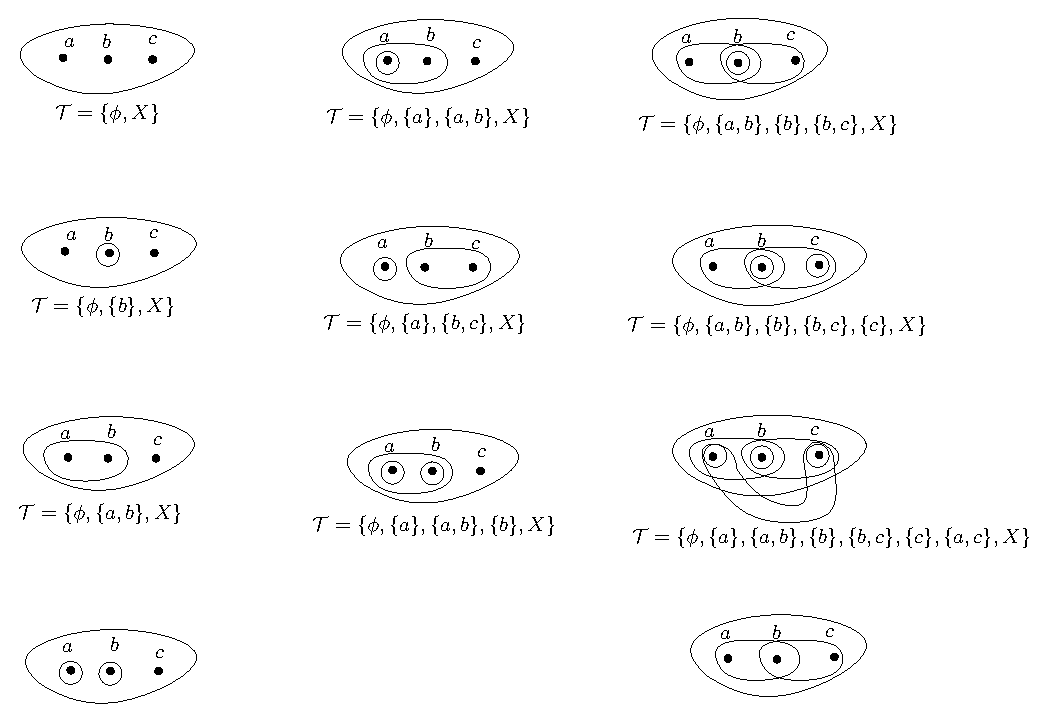
\includegraphics[height=3.5in]{fig133.eps}
\end{figure}

In the above, last two are not topologies.
\end{exmp}

\begin{exmp} 
 Let $X$ be a set and $\T_c=\{U\subseteq X: X \setminus U \text{ countable or } X \setminus U =X  \}$. Prove that $\T_c$ is a topology.
\end{exmp}
\begin{proof}
 
\end{proof}

\begin{defn}
 Let $\T$, $\T'$ be topologies on set $X$. If $\T\subseteq\T'$, we say that $\T'$ is \textbf{finer} than $\T$, and if  $\T\varsubsetneq\T'$, then \textbf{strictly finer}, we say $\T$ is \textbf{coarser} or \textbf{strictly coarser} in these two cases, respectively. We say that $\T$ is comparable to $\T'$ if either
 $\T\varsubsetneq\T'$ or $\T' \varsubsetneq\T$.
\end{defn}
\begin{defn}
 If $\T\varsubsetneq\T'$, then we say that $\T'$ is \textbf{larger} than $\T$, and $\T$ is \textbf{smaller} than $\T$
\end{defn}

\section{Basis for a Topology}
\begin{defn}
 If $X$ is a set, a \textbf{basis} for a topology on $X$ is a collection $\mathcal{B}$ of subsets of $X$ (called \textbf{basis} elements) such that 
 \begin{enumerate}
  \item $\forall x\in X, \exists B\in \mathcal{B}$ such that $x\in \mathcal{B}$.
  \item If $x\in B_1\bigcap B_2$, where $B_1, B_2 \in \mathcal{B}$ then $\exists B_3 \in \mathcal{B}$ such that $x\in B_3\subseteq B_1\bigcap B_2$.
 \end{enumerate}
\end{defn}
 If $\mathcal{B}$ satisfies these two conditions, we define the topology $\T$ generated by $\mathcal{B}$ as follows. A subset $U$ of $X$ is called open in $X$ if for each $x\in U, \exists B\in \mathcal{B}$ such that $x\in B\varsubsetneq U$. 
 Note: $\mathcal{B}\subseteq\T$.
 
 Next, we prove that the collection $\T$ generated by basis $\mathcal{B}$ is indeed a topology on $X$. First, we check that both $\emptyset$ and $X$ belongs to $\T$. Let $U$ be an empty set, in this case $U$ vacuously belongs to $\T$. Similarly $\forall x\in X, \exists B$ such that $x\in B\varsubsetneq X$. Next, to prove that the union of the elements of any sub-collection of $\T$ is in $\T$, we take an indexed family $\bigcup_{i\in \mathcal{I}}U_i$ of elements of $\T$  and show that $\bigcup_{j\in \mathcal{J}}U_j$ is in $\T$. For each $x\in U$, there exists index $j\in J$ such that $x\in U_j$. Since $U_j \varsubsetneq \T$ there exists basis element $B$ such that $x\in B$ and $B\varsubsetneq U_j$. Thus $x\in B$ and $B\varsubsetneq U$, so $U\varsubsetneq\T$ by definition. 
 
 Let $U_1$ and $U_2$  be finite sub-collections of $\T$. Now, first we want to show that $U_1\bigcap U_2 $ belongs to $\T$. Let $x\in U_1\bigcap U_2 $, we can choose a basis elements $B_1$ and $B_2$ such that $x\in B_1$ and $x\in B_2$, also $ B_1\varsubsetneq U_1$ and $B_2\varsubsetneq U_2$. Using the second condition in the definition of the basis we can choose a basis element $B_3$ such that $x\in B_3$ and $B_3\varsubsetneq B_1\bigcap B_2$. Then $x\in B_3$ and $B_3\varsubsetneq U_1\bigcap U_2$, thus $U_1\bigcap U_2$ belongs to $\T$, by definition. Using induction we can show that any arbitrary intersection belongs to $\T$.

\begin{figure}[!h]
 \centering
 \includegraphics[height=2in]{fig134.eps}
\end{figure}

\begin{exmp}
 As shown in above figure, consider the collection of all circular regions (interiors of circles) $\mathcal{B}$. $\mathcal{B}$ is a basis. 
\end{exmp}
\begin{exmp}
 $\mathcal{B}'$ collection of rectangular elements is also a basis. 
\end{exmp}
\begin{exmp}
 Let $X$ be any set, then collection of all singletons is basis for \textbf{discrete topology} on $X$.
\end{exmp}
 \begin{lem}
Let $X$ be a set, and $\mathcal{B}$ be a basis for topology $\T$ on $X$. Then $\T$ equals the collection of all unions of elements of $\mathcal{B}$.
\end{lem}
\begin{proof} Since $\mathcal{B}\varsubsetneq\T$ and $\T$ is a topology then collection of all union of $\mathcal{B}$ is in $\T$. Now, we have to show $\T\subseteq \text{ collection of all union of elements of } \mathcal{B}$. Let $U\in \T$, let $x\in U$, choose $B_x\in \mathcal{B}$ such that $x\in B_x\subseteq U$. Then $U=\bigcup_{x\in U}B_x$.
\end{proof}


\end{document}  